\chapter{Algorithmen zum Zeichnen von Bäumen}
\label{chap:kapitel3}
Im Folgenden werden drei verschiedene Algorithmen zum Zeichnen von Bäumen im Ebenen-Layout vorgestellt. Wie in Kapitel \ref{chap:einleitung}
bereits angekündigt, wird jeweils auf den Ablauf, einer eigenen Implementierung in Java und auf die Vor- und Nachteile eingegangen. Ziel wird
es sein, Verständnis für diese Algorithmen zu schaffen.

\section{Naiver Algorithmus von Wetherell und Shannon}
\erstelltvon{Garan}

Das Paper “Tidy Drawings of Trees” von Charles Wetherell und Alfred Shannon aus dem Jahre 1979, 
welches im IEEE Trans. Softw. Eng. erschienen ist, handelt von verschiedenen Algorithmen zum Zeichnen von Bäumen\cite[]{q1}.
Der erste Algorithmus, der von den beiden Autoren beschrieben und vorgestellt wird, ist ein naiver Algorithmus 
zum Zeichnen von Bäumen. Dieser Algorithmus soll dabei zwei Anforderungen erfüllen. Die erste Anforderung wird dabei
an die Ästhetik des gezeichneten Baumes gestellt. 
\begin{quotation}
	\textit{Aesthetic 1:} Nodes of a tree at the same height should lie
	along a straight line, and the straight lines defining the levels
	should be parallel \cite[]{q1}.
\end{quotation}
Alle Knoten, die dieselbe Höhe haben, sollen sich auf einer horizontalen
Linie befinden. Jede Höhe hat dabei eine Linie, auf welcher sich die Knoten befinden sollen und diese Linien sollen alle
parallel zueinander sein. Außerdem soll der Algorithmus beim Zeichnen eines Baumes ein physikalisches Limit einhalten:
\begin{quotation}
	\textit{Physical limit:} Tree drawings should occupy as little width
	as possible (the height of a tree drawing is fixed by the tree
	itself) \cite[]{q1}.
\end{quotation}
Das bedeutet, dass der Algorithmus möglichst schmale Bäume zeichnen soll. Jedoch wird die Höhe des Baumes durch diese Anforderungen
nicht eingeschränkt. Stattdessen ist die Höhe durch den Baum vorgegeben \cite[]{q1}.

\label{chap:kapitel3_1_Ablauf}
\subsection{Ablauf}
\erstelltvon{Treulieb}
Bevor die Funktionsweise des Algorithmus beschrieben werden kann, muss die Baumstruktur 
wie folgt definiert sein: Sie benötigt eine Struktur die symbolisch für ein Knoten des Baums steht. 
Diese Knoten-Struktur muss hierbei ihren Vater kennen, auf ihre Kinder zugreifen können sowie ihre Position und
Höhe im Baum speichern können.

Dieser Algorithmus besitzt zwei Eingabeparameter: Die Wurzel und die Höhe des Baumes.
Die Wurzel muss hierbei vom Typ der zuvor definierten Struktur sein. Zu Beginn wird eine Variable definiert:
Ein Array (später Positions-Array genannt), welches die jeweils nächste freie X-Position einer Ebene des Baums beinhaltet.
Hiernach wird über die Baumstruktur der Wurzel, in der Pre-Order-Traversierung, traversiert.
Nun werden die X- und Y-Attribute der Knoten wie folgt bestimmt und gesetzt:

Der derzeitige Knoten bekommt als X-Position den Wert aus dem Positions-Array, in Abhängigkeit von seiner Höhe im Baum.
Danach wird die Zahl im Positions-Array inkrementiert. Die Y-Position des Knoten wird nun in Abhängigkeit zur Höhe des Knoten
mit der folgenden Formel berechnet: $$y := 2 * HoeheDesKnotens + 1$$

Dieses Vorgehen wird nun für alle Knoten in dem Baum wiederholt. 

Nach dem Durchlaufen aller Knoten des Baumes sind alle X- und Y-Koordinaten gesetzt und der Baum kann gezeichnet werden.

\subsection{Implementierung in Java}
\erstelltvon{Treulieb}
Dieser Algorithmus wurde in Java implemeniert. Hierzu wurde die zuvor vorgestellte Datenstruktur
implementiert. Zusätzlich wurden Methoden hinzugefügt, die beispielsweise
ein einfaches Traversieren über den Baum ermöglichen oder zum Setzen von Kindern.

Diese Klasse sieht wie folgt aus:

\begin{lstlisting}[caption=Vereinfachte Implementierung der Knotenklasse, label=code:knotenclass]
class Knoten {
	private Knoten father;
	private Knoten[] childs;
	private int hoehe;
	private int x, y;
	private char data;

	public void traversPreOrder(Consumer<Knoten> cons) { /*...*/ }

	public void setChilds(Knoten... childs) { /*...*/ }

	// Getter, Setter, weitere Hilfsmethoden...
}
\end{lstlisting}

Nachdem diese Klasse erstellt wurde, kann der Algorithmus als Prozedur implementiert werden.
Hierzu wurde eine Prozedur namens \glqq algorithmus1\grqq erstellt, die zwei Parameter besitzt: Der Wurzel-Knoten
und die Höhe des Baums. Die weitere Implementierung wird, wie zuvor beschrieben, durchgeführt. Eine mögliche Implementierung
kann wie folgt aussehen:

\begin{lstlisting}[caption=Implementierung des naiven Algorithmus]
public static void algorithmus1(Knoten wurzel, int maximaleHoehe) 
{
	int[] nextX = new int[maximaleHoehe];
	for(int i = 0; i < nextX.length; i++)
		nextX[i] = 1;
	
	wurzel.traversPreOrder(knoten -> {
		knoten.setX(nextX[knoten.getHoehe()]);
		knoten.setY(2 * knoten.getHoehe() + 1);
		
		nextX[knoten.getHoehe()] += 1;
	});
}
\end{lstlisting}

Wird diese Prozedur mit einer Baumstruktur aufgerufen, so werden alle X- und Y-Koordinaten gesetzt.
Ein Beispiel für einen gezeichneten Baum kann in der Abbildung \ref{pic:baum_algo_1} betrachet werden.

\begin{figure}[H]
    \centering
    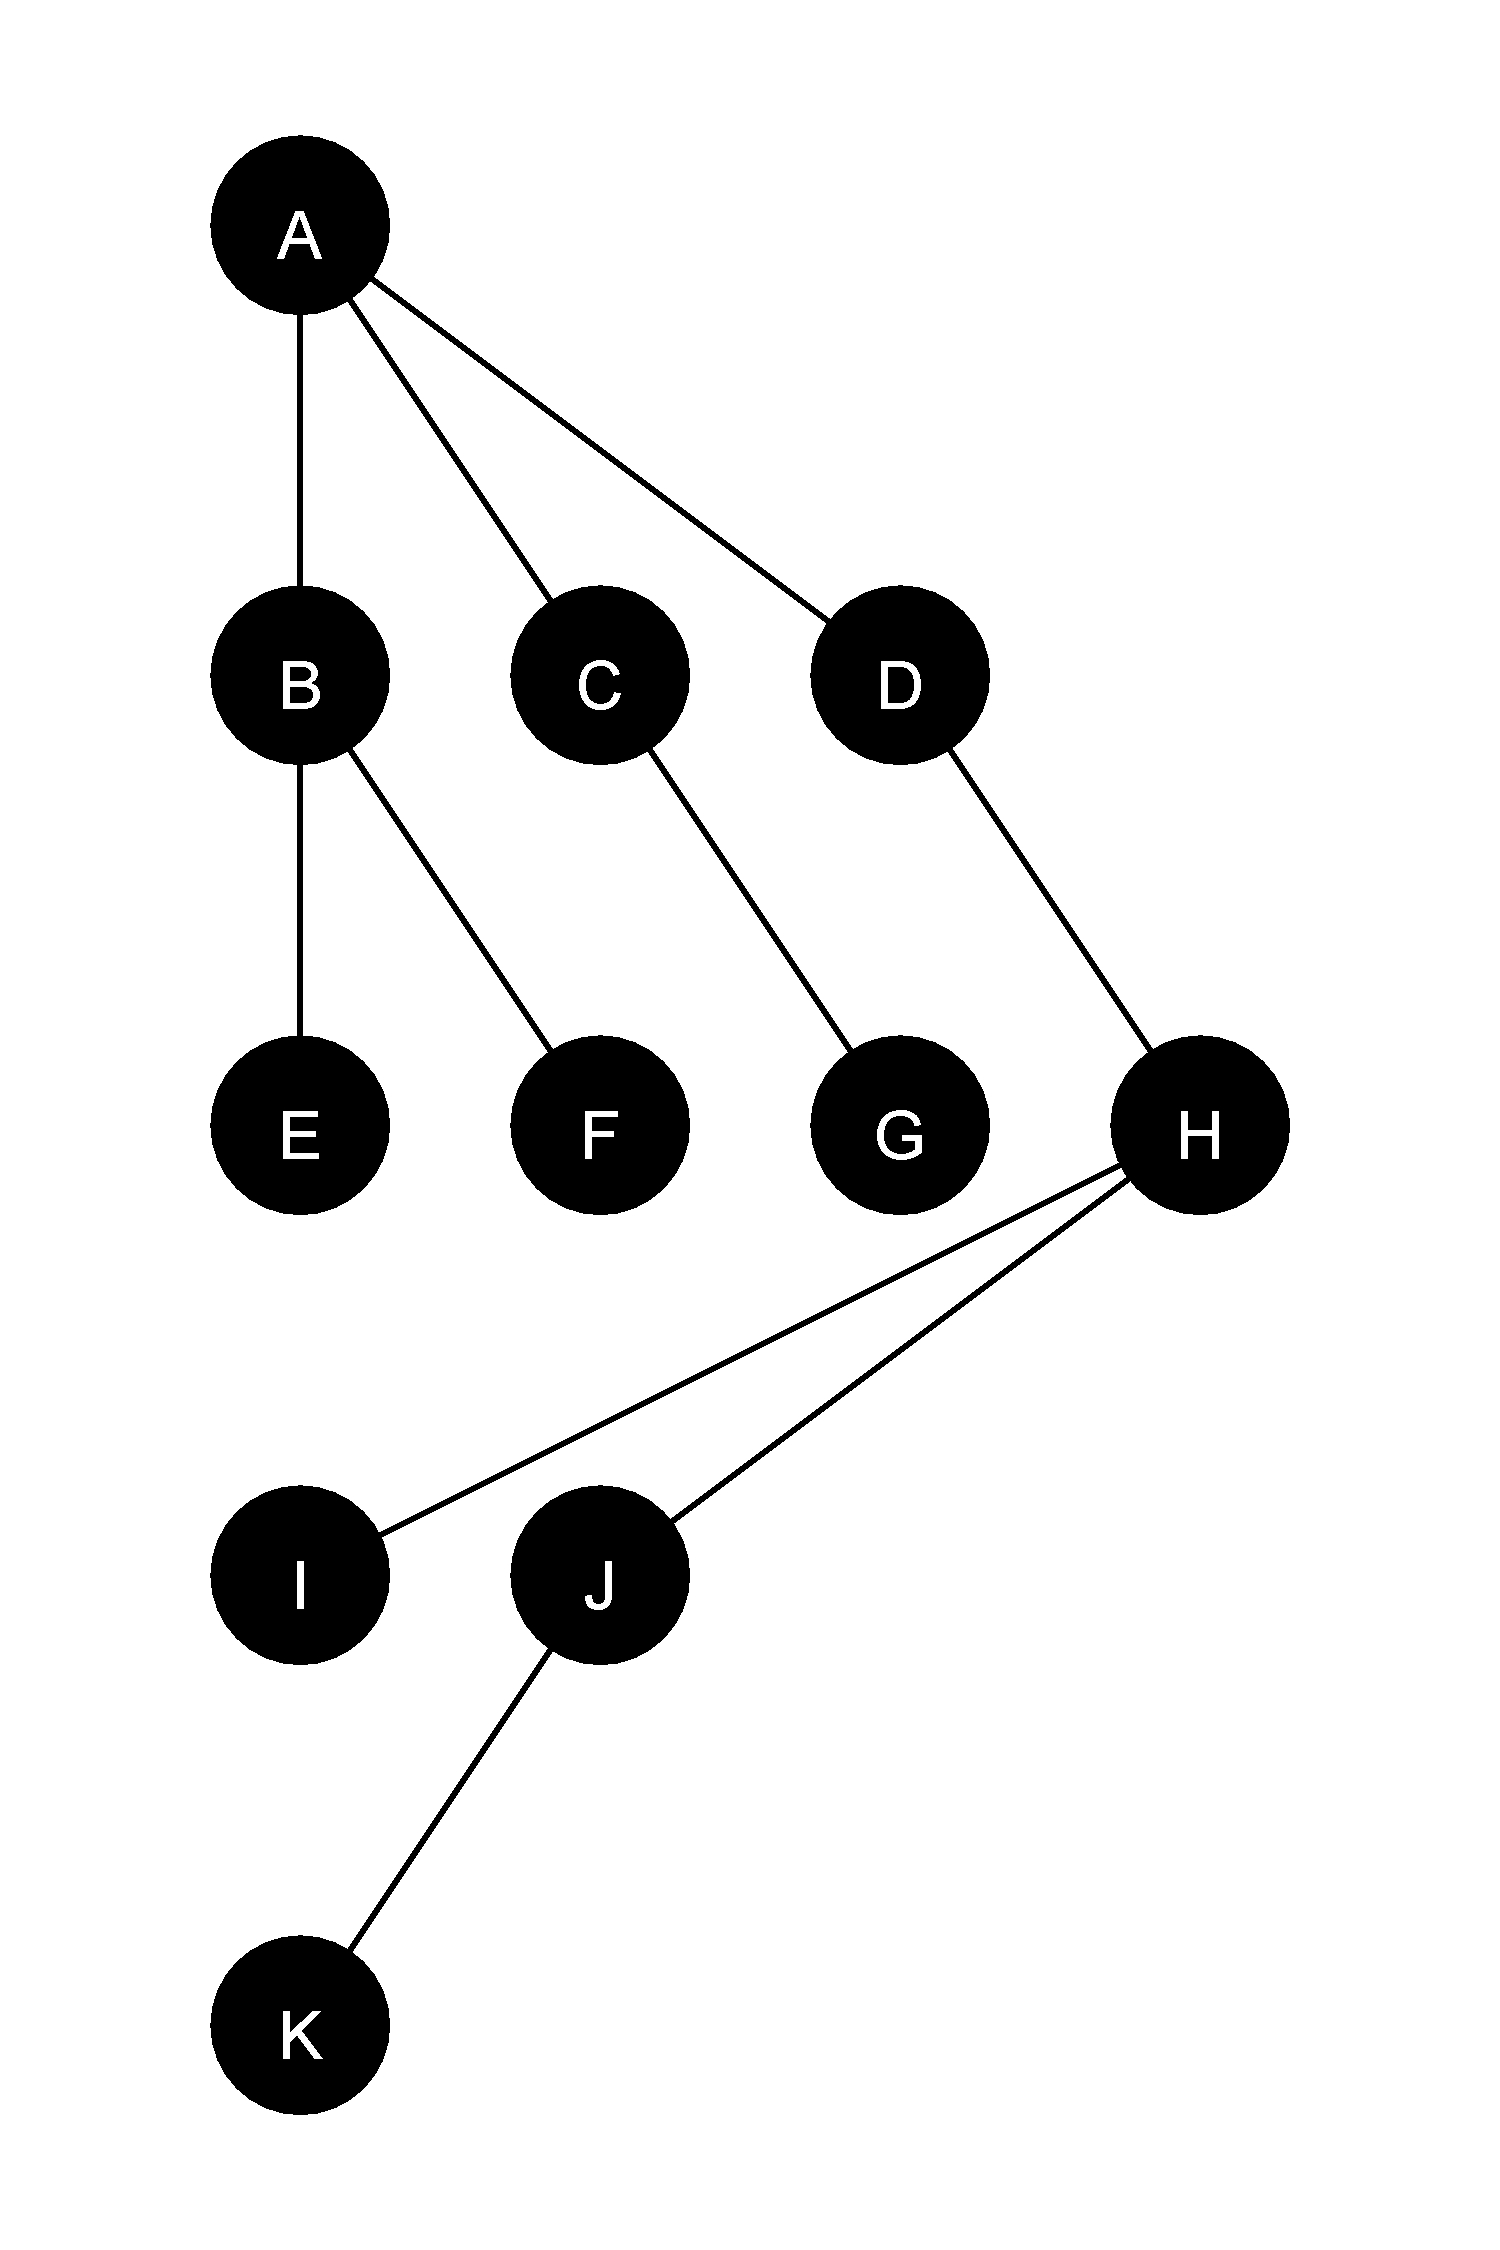
\includegraphics[width=7cm, height=10cm]{abbildungen/baum_algo_1}
    \caption{Gezeichneter Baum durch den ersten Algorithmus}
    \label{pic:baum_algo_1} 
\end{figure}

\subsection{Vor- und Nachteile}
\erstelltvon{Garan}
Die Abbildung \ref{pic:baum_algo_1} zeigt einen Baum, welcher von unserer Java-Implementierung des naiven Algorithmus von Wetherell und Shannon
gezeichnet wurde.
Auf dem ersten Blick wird deutlich, dass dieser gezeichnete Baum maximal schmal ist, da jeder Knoten so weit links wie möglich steht.
Diese Eigenschaft wird aber nur auf Kosten der Übersichtlichkeit erfüllt. Bei der Beziehung zwischen H als Vater und I und J als Sohn wird 
deutlich, dass der von diesem Algorithmus gezeichnete Baum unübersichtlich ist. Außerdem sagt die Position der Knoten nichts über die Daten 
aus, welche die Knoten beinhalten könnten. Egal ob die Daten, welche I und J beinhalten, größer oder kleiner als die Daten in H wären, 
sie würden trotzdem an der selben Position stehen. 
Deshalb definieren Wetherell und Shannon weitere Anforderungen, die Algorithmen zum Zeichnen von Bäumen erfüllen müssen.

